% The scene of the imaging sonar how-to (docs/how-to/sonar-imaging.md), world gz_sonar/worlds/sonar_imaging.sdf.
% World frame: x forward, y to port, z up, meters. Seabed z = -5, surface z = 0.
% BlueROV2 at (0, 0, -2.5), level; ECHO imaging sonar at (0.25, 0, -2.38), pitched down 15 deg; 120 x 20 deg (-3 dB),
% range 0.2 to 15 m. Height above the seabed 2.62 m: the axis meets the seabed 9.8 m ahead, the lower -3 dB edge
% (25 deg down) at 6.2 m slant, and rays 30 deg below the axis (45 deg down) at 3.7 m slant, where the seabed first
% shows faintly. Targets: glass float r 0.2 at (6.5, -1.5); steel cylinder r 0.15 x 0.6, axis along x then yawed
% 0.5 rad, at (7, 0); concrete block 0.5 m cube, yaw 0.3, at (7.5, 1.5); tire r 0.35 x 0.25 lying flat at (9.5, -1);
% marker flag, 2 m pole with a 0.5 x 0.3 flag toward +y, at (9, 1), acoustically transparent.
% (a) side view, x to the right; (b) plan view, forward up and starboard (-y) right, as the sonar image is drawn.
% True scale in both.
% Build: pdflatex sonar_imaging_scene.tex, then pdftocairo to ../../how-to/images/sonar-imaging-scene.{png,svg}
\documentclass[tikz,border=6pt]{standalone}
\usetikzlibrary{arrows.meta,calc}
\renewcommand{\familydefault}{\sfdefault}
\tikzset{
  lbl/.style={font=\sffamily\small},
  beam/.style={fill=black!7,draw=black,thin},
  dim/.style={thin,{Latex[length=1.6mm]}-{Latex[length=1.6mm]}},
  lead/.style={thin,black!70},
  axis/.style={thin,dashed},
  ghost/.style={black!45,densely dashed},
  % where a ray at elevation e (relative to the axis) and azimuth a meets the seabed, sonar 2.62 m up, pitched 15 down
  declare function={
    wx(\e,\a)=cos(15)*cos(\e)*cos(\a)+sin(15)*sin(\e);
    wy(\e,\a)=cos(\e)*sin(\a);
    wz(\e,\a)=-sin(15)*cos(\e)*cos(\a)+cos(15)*sin(\e);
    gx(\e,\a)=0.25-2.62/wz(\e,\a)*wx(\e,\a);
    gy(\e,\a)=-2.62/wz(\e,\a)*wy(\e,\a);
  },
}
% seabed line from x0 to x1 at height z, two rows of dots below
\newcommand{\seabed}[3]{
  \draw[thick] (#1,#3) -- (#2,#3);
  \foreach \r [count=\i] in {0.1,0.25} {
    \pgfmathsetmacro{\o}{mod(\i,2)*0.1}
    \pgfmathsetmacro{\n}{int((#2-#1-0.25)/0.2)}
    \foreach \k in {0,...,\n} \fill ({#1+0.1+\k*0.2+\o},{#3-\r}) circle (0.4pt);
  }
}

\begin{document}
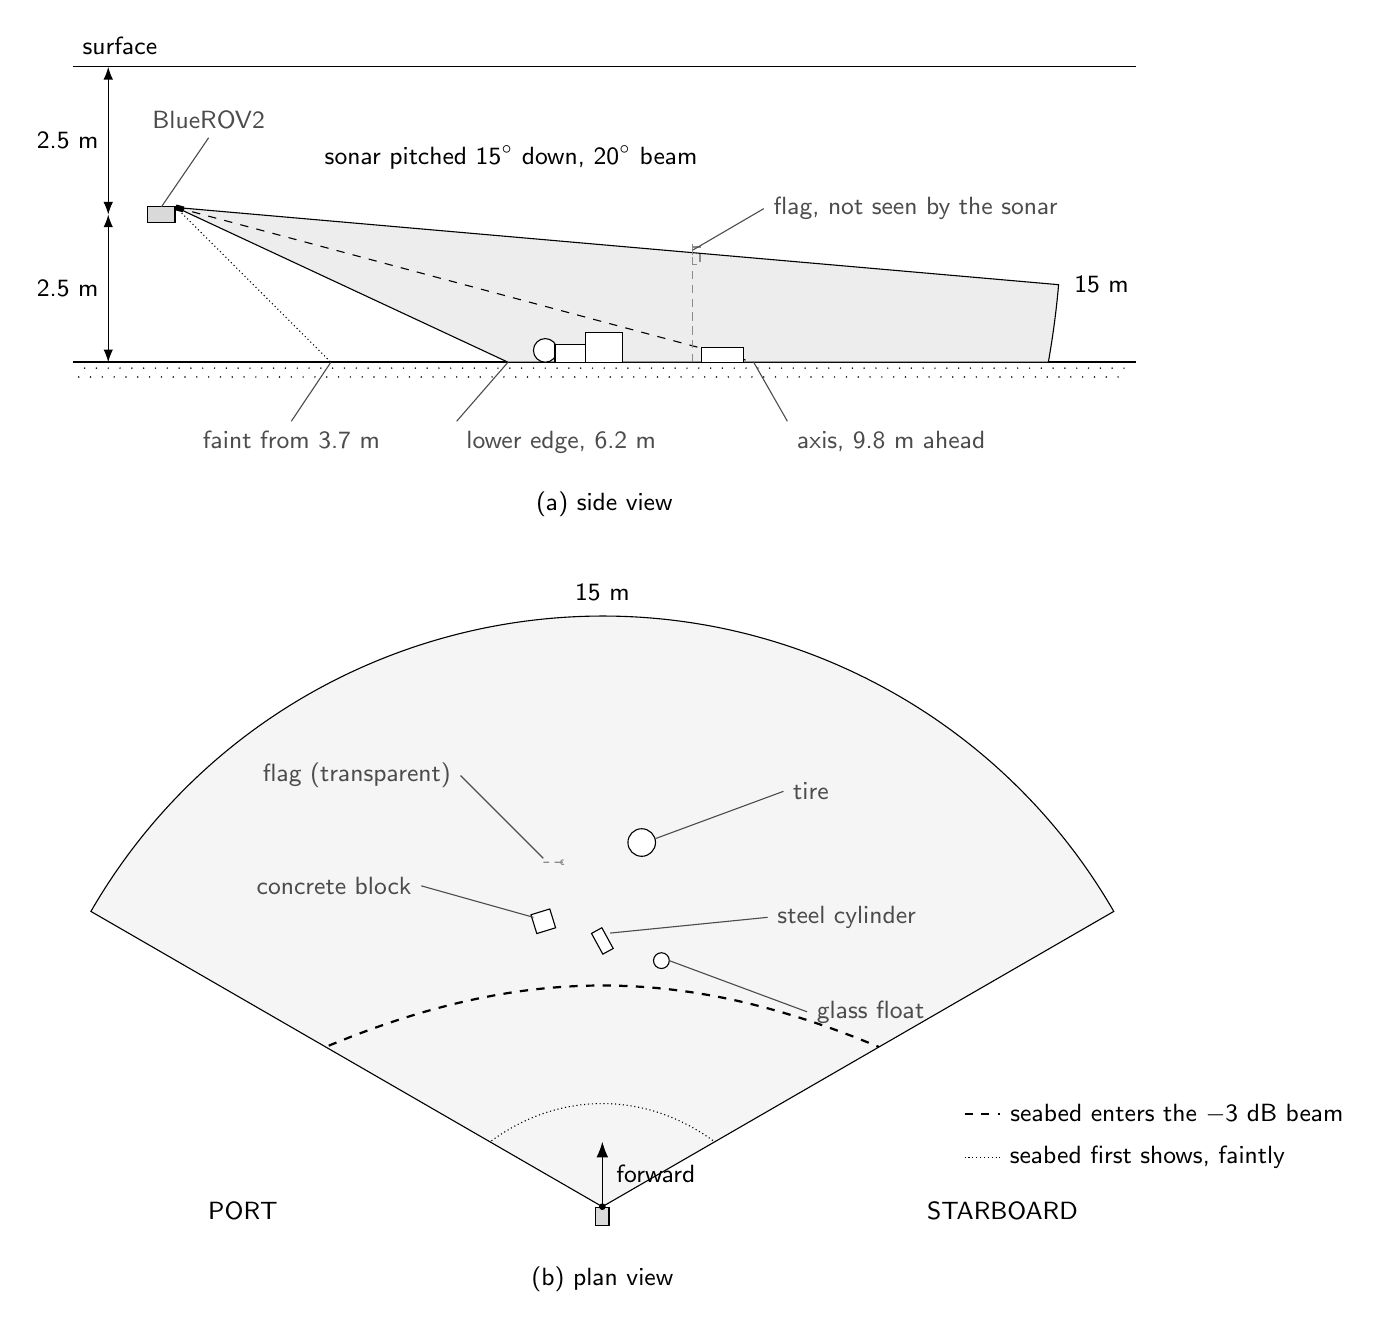
\begin{tikzpicture}
  % ================================================ (a) side view
  \begin{scope}[scale=0.75]
    \def\zs{-2.38}
    \pgfmathsetmacro{\af}{asin(2.62/15)}
    \draw[thin] (-1.5,0) -- (16.5,0);
    \node[lbl,anchor=south west] at (-1.5,0.05) {surface};
    \seabed{-1.5}{16.5}{-5}
    % the -3 dB beam: 5 to 25 deg down, out to 15 m or the seabed
    \draw[beam] (0.25,\zs) -- ({0.25+15*cos(5)},{\zs-15*sin(5)}) arc (-5:-\af:15) -- ({0.25+2.62/tan(25)},-5) -- cycle;
    \draw[axis] (0.25,\zs) -- ({0.25+2.62/tan(15)},-5);
    \draw[thin,densely dotted] (0.25,\zs) -- ({0.25+2.62},-5);
    % targets, projected onto the x-z plane
    \draw[fill=white] (6.5,-4.8) circle (0.2);
    \draw[fill=white] ({7-0.3*cos(28.65)-0.15*sin(28.65)},-5) rectangle ({7+0.3*cos(28.65)+0.15*sin(28.65)},-4.7);
    \draw[fill=white] ({7.5-0.25*(cos(17.2)+sin(17.2))},-5) rectangle ({7.5+0.25*(cos(17.2)+sin(17.2))},-4.5);
    \draw[fill=white] (9.15,-5) rectangle (9.85,-4.75);
    \draw[ghost] (9,-5) -- (9,-3) (9,-3.05) rectangle (9.12,-3.35);
    % ROV and sonar
    \draw[fill=black!15] (-0.23,-2.63) rectangle (0.23,-2.37);
    \begin{scope}[shift={(0.25,\zs)},rotate=-15]
      \draw[fill=black] (0,-0.04) rectangle (0.12,0.04);
    \end{scope}
    % dimensions and labels
    \draw[dim] (-0.9,0) -- (-0.9,-2.5) node[lbl,midway,left] {2.5 m};
    \draw[dim] (-0.9,-2.5) -- (-0.9,-5) node[lbl,midway,left] {2.5 m};
    \draw[lead] (0,-2.37) -- (0.8,-1.2) node[lbl,anchor=south] {BlueROV2};
    \node[lbl,anchor=south west] at (2.6,-1.9) {sonar pitched 15$^\circ$ down, 20$^\circ$ beam};
    \node[lbl,anchor=west] at ({0.25+15*cos(5)+0.1},{\zs-15*sin(5)}) {15 m};
    \draw[lead] ({0.25+2.62},-5) -- (2.2,-6.0) node[lbl,anchor=north] {faint from 3.7 m};
    \draw[lead] ({0.25+2.62/tan(25)},-5) -- (5.0,-6.0) node[lbl,anchor=north west] {lower edge, 6.2 m};
    \draw[lead] ({0.25+2.62/tan(15)},-5) -- (10.6,-6.0) node[lbl,anchor=north west] {axis, 9.8 m ahead};
    \draw[lead] (9,-3.1) -- (10.2,-2.4) node[lbl,anchor=west] {flag, not seen by the sonar};
    \node[lbl] at (7.5,-7.4) {(a) side view};
  \end{scope}

  % ================================================ (b) plan view, forward up, starboard right
  \begin{scope}[shift={(5.6,-14.6)},x={(0cm,0.5cm)},y={(-0.5cm,0cm)}]
    % the 120 deg fan out to 15 m, and where the seabed enters it
    \draw[beam,fill=black!4] (0.25,0) -- ({0.25+15*cos(60)},{15*sin(60)}) arc[start angle=150,end angle=30,radius=7.5cm]
          -- cycle;
    \begin{scope}
      \clip (0.25,0) -- ({0.25+15*cos(60)},{15*sin(60)}) arc[start angle=150,end angle=30,radius=7.5cm] -- cycle;
      \draw[thin,densely dotted] plot[domain=-62:62,samples=41] ({gx(-30,\x)},{gy(-30,\x)});
      \draw[thick,dashed] plot[domain=-62:62,samples=41] ({gx(-10,\x)},{gy(-10,\x)});
    \end{scope}
    % targets at true size
    \draw[fill=white] (6.5,-1.5) circle (0.2);
    \draw[fill=white,rotate around={28.65:(7,0)}] (6.7,-0.15) rectangle (7.3,0.15);
    \draw[fill=white,rotate around={17.2:(7.5,1.5)}] (7.25,1.25) rectangle (7.75,1.75);
    \draw[fill=white] (9.5,-1) circle (0.35);
    \draw[ghost] (9,1) circle (0.06) (9,1) -- (9,1.5);
    % ROV
    \draw[fill=black!15] (-0.23,-0.17) rectangle (0.23,0.17);
    \fill (0.25,0) circle (1.2pt);
    % labels
    \draw[lead] (6.5,-1.7) -- (5.2,-5.2) node[lbl,anchor=west] {glass float};
    \draw[lead] (7.2,-0.2) -- (7.6,-4.2) node[lbl,anchor=west] {steel cylinder};
    \draw[lead] (7.6,1.75) -- (8.4,4.6) node[lbl,anchor=east] {concrete block};
    \draw[lead] (9.6,-1.35) -- (10.8,-4.6) node[lbl,anchor=west] {tire};
    \draw[lead] (9.1,1.5) -- (11.2,3.6) node[lbl,anchor=east] {flag (transparent)};
    \node[lbl,anchor=south] at (15.4,0) {15 m};
    \node[lbl,anchor=north east] at (0.6,8) {PORT};
    \node[lbl,anchor=north west] at (0.6,-8) {STARBOARD};
    \draw[-{Latex[length=2mm]}] (0.25,0) -- (1.9,0) node[lbl,midway,anchor=west] {\,forward};
    \draw[thick,dashed] (2.6,-9.2) -- ++(0,-0.9) node[lbl,anchor=west] {seabed enters the $-$3 dB beam};
    \draw[thin,densely dotted] (1.5,-9.2) -- ++(0,-0.9) node[lbl,anchor=west] {seabed first shows, faintly};
    \node[lbl] at (-1.6,0) {(b) plan view};
  \end{scope}
\end{tikzpicture}
\end{document}
